\newpage
\subsubsection{Dispersion Relations and Stability} \label{DispRelaStabSection}

\textcite{whitham1974linearnonlinear} explains that in wave propagation theory, a system of partial differential equations that governs the propagation properties of waves is encoded by the dispersion relation of the wave in the frequency and wave number space. The dispersion relation, then, is the functional relationship between the angular frequency $\omega$, and the wave number k. 


The propagation of a wave through a medium can be described by the acoustic wave equation, and a phasor solution using Euler's formula in the ansatz $A e^{\mathrm{i}\left(\omega t + \theta \right)}$ is sought after for exploring dispersion relations. For the three types of waves possible within the domain (acoustic, vorticity, and entropy), solutions exist in one-dimensional form as

\begin{equation} \label{eq:OGAnsatz}
\mathbf{U}\left(x,t\right)=\mathbf{A}e^{\mathrm{i}\left(\omega t - k_x x \right)}
\end{equation}
Again using the PML complex change of variable from Equation \ref{eq:ComplexChange}
\begin{displaymath}
    x \rightarrow x + \frac{\mathrm{i}}{\omega} \int^{x}_{x_0} \sigma_{x} \left( x \right) \ dx
\end{displaymath}
to give
\begin{equation} \label{disprelUequation}
    \mathbf{U}\left(x,t\right) = \mathbf{A}e^{-\frac{k_x}{\omega} \int^{x}_{x_0} \sigma_{x} \ dx} e^{\mathrm{i} \left(\omega t - k_x x \right)}
\end{equation}
 
 
The first exponential factor of Equation \ref{disprelUequation} is very telling of the coherency of the phase and group velocity. The $k/\omega$ term is the reciprocal of the phase velocity and so takes on its sign, and the $\int^x_{x_0}\sigma_x$ term indicates the direction of wave propagation - which takes on the sign of the group velocity ($\frac{\mathrm{d}\omega}{\mathrm{d}k}$). Given these two signs are the same, the exponential will retain it's negative power and continue to exponentially decay the wave. That is to say, the amplitude of the wave will decrease within the PML zone. The required condition is poetically summarised as $\frac{k}{\omega}\frac{\mathrm{d}\omega}{\mathrm{d}k}>0$ \cite{hu2005aPML}. The condition can be met by introducing a space-time transformation which aligns the phase and group velocities. The impact of which will be investigated as follows.
 
The dispersion relation for an acoustic wave supported by the Euler equations is
\begin{equation}
    \left(\omega - M k_x \right)^2 - k_x^2 = 0
\end{equation}
 
and when substituted with the non-transformed complex change of variables $k_x \rightarrow \frac{k_x}{1 + \frac{\mathrm{i} \sigma_x}{\omega}}$, becomes
 
 \begin{equation} \label{eq:UnstableDisp}
     \left(\omega - M \frac{k_x}{1+\frac{\mathrm{i} \sigma_x}{\omega}} \right)^2 - \left(\frac{k_x}{1+\frac{\mathrm{i} \sigma_x}{\omega}}\right)^2=0
 \end{equation}
 
Equation \ref{eq:UnstableDisp} is solved for the complex roots of $\omega$, of which the maximum growth rates $\omega_i$ (the imaginary parts) are plotted as a function of freestream Mach number $M$ and $x-$layer damping coefficient $\sigma_x$, for wavenumbers in the range $0<k_x<5$ - as seen in Figure \ref{fig:UnstableSigmaxM}. The growth rate is shown to increase with both freestream Mach and damping coefficient, with positive imaginary components. This indicates numerical instabilities with the illustrated combinations.

\begin{figure}[h!]
\centering
\makebox[0pt]{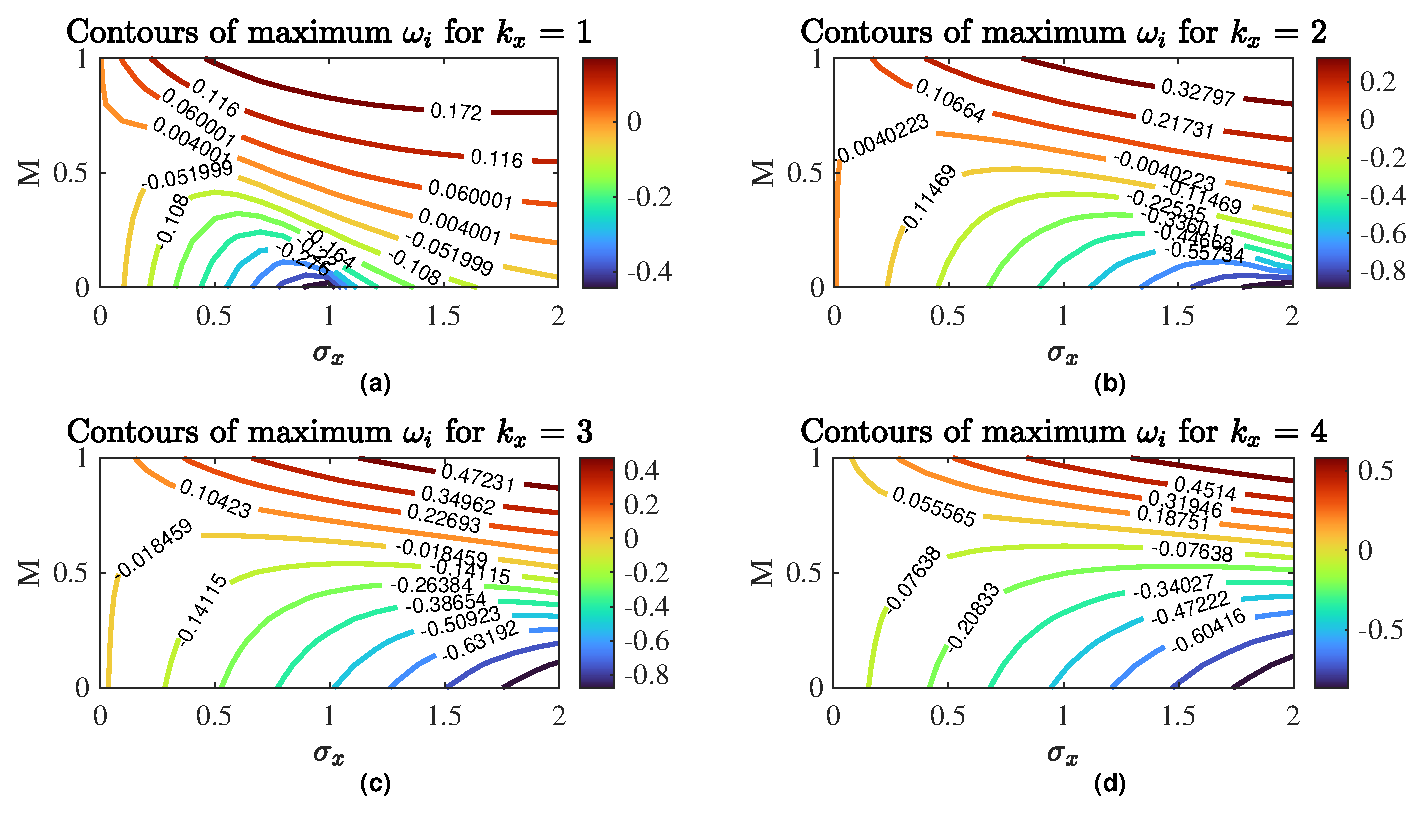
\includegraphics[width=14cm]{Figures/TechnicalAchievement/PMLBC/UnstableSigmaxM.eps}}
\caption{Contours of maximum growth rate, $\omega_{i}$, of numerically solved roots of non-transformed dispersion relation Equation \ref{eq:UnstableDisp}. Roots are a function of freestream Mach number $M$ and damping coefficient $\sigma_x$, for wavenumbers in the range $0 < k_{x} < 5$. N.B. colourbars have different scales for each subplot and are purely for visual reference to show positive \& negative roots.}
\label{fig:UnstableSigmaxM}
\end{figure}

Using the aforementioned space-time transformation from $\left(x,t\right)$ to $\left(\Bar{x},\Bar{t}\right)$, the corresponding wavenumbers and frequency are given by $\Bar{k}_x = k_x + \frac{M}{1-M^2}\omega$, $\Bar{\omega}=\omega$. Substituting these into the complex change of variables gives

\begin{equation}
    k_x \rightarrow \frac{k_x}{1 + \frac{\mathrm{i} \sigma_x}{\omega}} \left( k_x + \frac{M}{1-M^2}\omega\right) - \frac{M}{1-M^2}\omega
\end{equation}

which can then be substituted into Equation \ref{eq:UnstableDisp} and simplified to give

\begin{equation} \label{eq:StableDisp}
    \frac{\left( \omega + \mathrm{i} \sigma_x \right)^2}{\left(1-M^2\right)^2} - \left(k_x + \frac{M}{1-M^2}\omega\right)^2 - \frac{1}{1-M^2}\left(\omega + \mathrm{i} \sigma_x \right)^2 = 0
\end{equation}

Equation \ref{eq:StableDisp} is then solved similarly to Equation \ref{eq:UnstableDisp} to provide Figure \ref{fig:StableSigmaxM}, where it can be seen that only negative imaginary components exist for all shown combinations of freestream Mach and $x-$layer damping coefficient. Symbolic calculations for the same stability proof are shown in the appendix of \cite{hu2001astablePML}. This therefore proves the group/phase velocity instability is inhibited whenever the space-time transformation is included in the complex change of variables derivation.


\begin{figure}[h!]
\centering
\makebox[0pt]{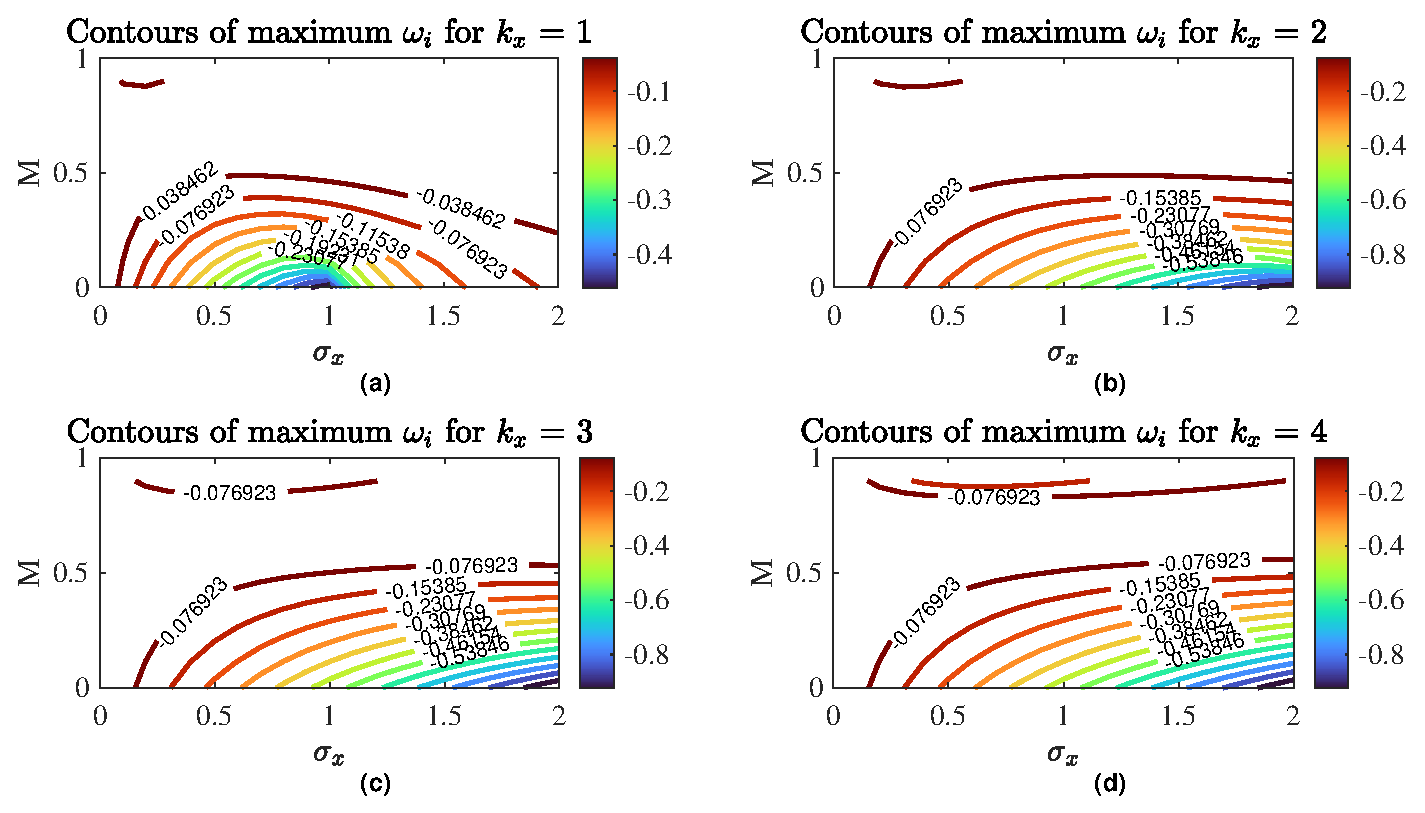
\includegraphics[width=14cm]{Figures/TechnicalAchievement/PMLBC/StableSigmaxM.eps}}
\caption{Contours of maximum growth rate, $\omega_{i}$, of numerically solved roots of space-time-transformed dispersion relation Equation \ref{eq:StableDisp}. Roots are a function of freestream Mach number $M$ and damping coefficient $\sigma_x$, for wavenumbers in the range $0 < k_{x} < 5$. N.B. colourbars have different scales for each subplot and are purely for visual reference to show all negative roots.}
\label{fig:StableSigmaxM}
\end{figure}


On another stability note, \textcite{tam1998pmlopenducted} describe how the PML boundary condition is not suitable for internal ducted flows as a boundary condition as it supports unstable solutions - the highly dispersive nature of the duct modes leads to a stripe of transmitted waves in the PML which are amplified rather than exponentially damped. The transmitted waves are long (not short component) and so are not actively suppressed by any kind of artificial selective damping \cite{tam2012computational} that might be implemented in a more complete solver. Nonetheless, this specific instability is confined to internal ducted flows and does not present itself for more open domain problems, which this boundary condition is proposed for (gas turbine noise prediction).